\chapter{Application Design}

This chapter details the user interface and design elements of the application, specifically how the application appeared when the user testing took place. It details the design decisions made and then proceeds to explain and justify why it was thought that making these decisions would improve the user experience.

\section{Category and Experience Selection}

When the user first connects to the web application, they are shown the view in Figure \ref{fig:view1}. This view allows them to input their experience with German, as well as selecting the category of article that they wish to read. Four different experience levels are available, 'beginner', 'intermediate', 'advanced' and 'near fluent'. The decision to categorize language experience like this was made as these different experience levels are in English and are commonly used as descriptions of language proficiency. While it would have been possible to use much more formal definitions of language proficiency, for example the Common European Framework of Reference for Language (CEFRL), these definition are not commonly taught and would most likely confuse a large proportion of users. Once 'beginner', 'intermediate' and 'advanced' had been decided upon, the decision was made to add a forth level 'near fluent' to distinguish between users who needed barely any help and users who needed some help. It was also believed that fluent German speakers would have no need to use the application, and therefore did not need to be considered when selecting these levels.

\begin{figure}
	\caption[Screenshot of the Category Selection View]{Screenshot of the category selection view, where the user inputs the category of article they want to read, as well as their experience level.}
	\label{fig:view1}
	\begin{center}
	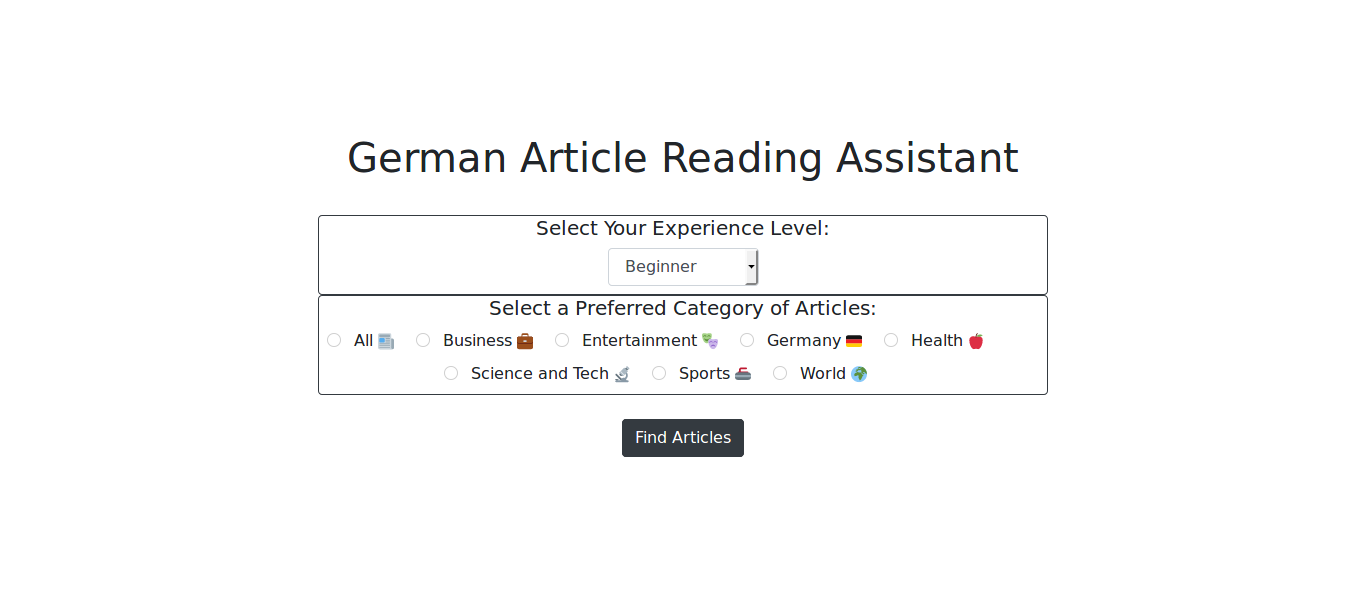
\includegraphics[width=\textwidth]{Graphics/View1}
	\end{center}
\end{figure}

The user then goes on to select a category of article based on their interests. The selections available are 'All', 'Business', 'Entertainment', 'Germany', 'Health', 'Science and Tech', 'Sports' and 'World'. These categories were chosen to reflect traditional news categories that one would find on a news website. The application originally used German titles for the categories, but they were switched to English as it was believed that some users would not be skilled enough in German to understand the meaning of the titles without access to translations, which are not currently available on this screen. 

An emoji was added next to the name for each category, primarily to make it easier to identify the categories upon sight, but also to broaden the colour pallet being used in the application.

The initial prototype of the application had a different article selection view, where the URL of the desired article was inputted instead of a category selection screen. This had both advantages and disadvantages over the current selection model in the final application. This earlier version allowed the user to find articles that interested them and then input them into the application and continue reading there, but it also relied on the user having the ability  to find articles that interested them externally. Ideally, it would have been best to have both the category selection and direct article input methods implemented with different input screens.

\section{Article Selection}

Once the user has inputted their ability level and desired category of article, they are then presented with the view shown in Figure \ref{fig:view2}. This is a list of articles in the selected category, with titles in German, followed by a difficulty rating. Titles are left in the original German as the user can determine any words that that they do not know from context, making it easier than the category names to determine. If the user cannot figure out the title, the difficulty ratings provide a clear indication of the level of the articles, suggesting which ones would be suitable for them. 

\begin{figure}
	\caption[Screenshot of the Article Selection View]{An example of the article selection view, here the user is shown a list of articles in their selected category as well as the difficulty rating for each article. They then go on to select an article from the list.}
	\label{fig:view2}
	\begin{center}
	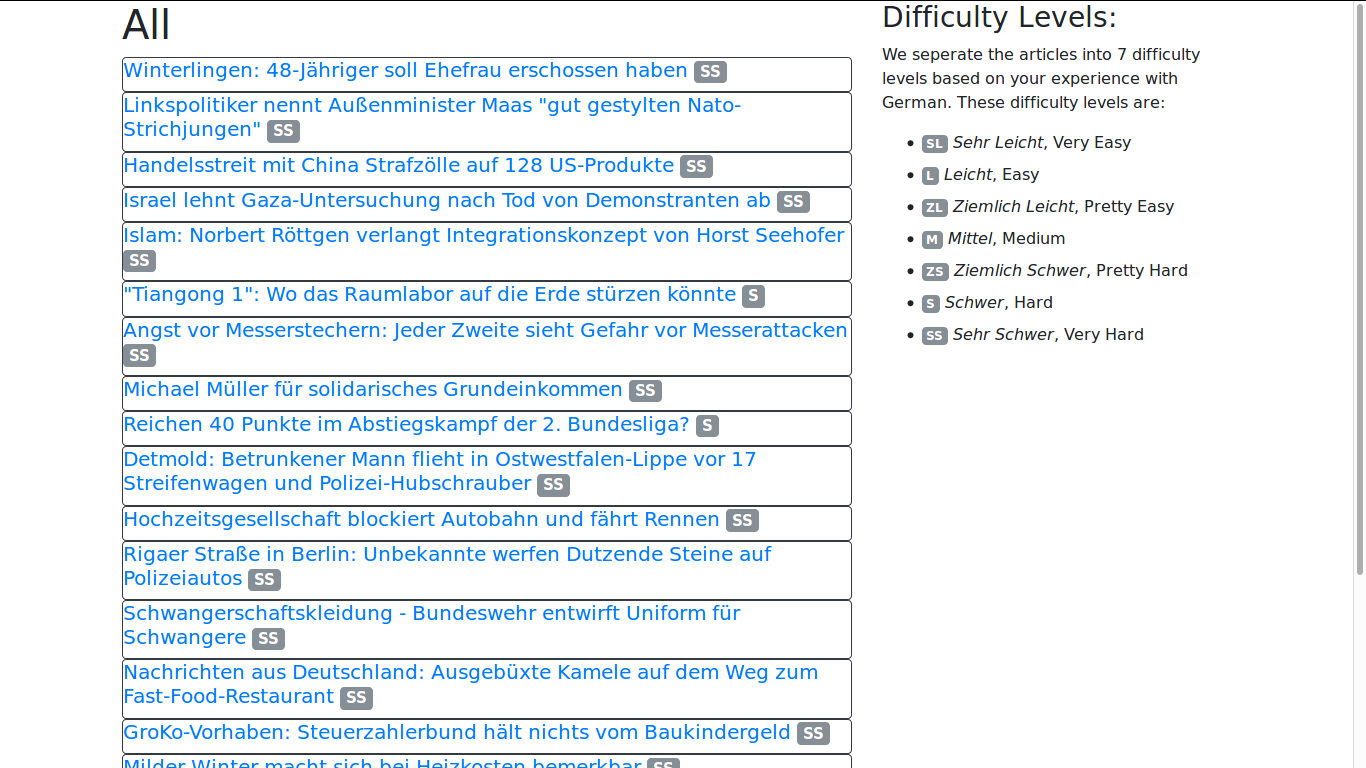
\includegraphics[width=\textwidth]{Graphics/View2}
\end{center}
\end{figure}

To the right of the list of articles, in the position where the gloss will be in the article view, a list of definitions of the different difficulty rating can be seen. These, going in order from most difficult to least, are 'SS', 'S', 'ZS', 'M', 'ZL', 'L' and 'SL'. These difficulty ratings were chosen as they are acronyms of the German phrases 'Sehr Schwer', 'Schwer', 'Ziemlich Schwer', 'Mittel', 'Ziemlich Leicht' 'Leicht' and 'Sehr Leicht' respectively. These phrases translate to the appropriate difficult levels, each one of them having a unique acronym. Seven categories were used, expanding the standard 'Easy', 'Medium' and 'Hard' to include 'Very Hard', 'Somewhat Hard', 'Somewhat Easy' and 'Very Easy'. These categories can be placed easily on a scale by a user, and then be used to identify with a fair amount of precision how hard said user will find the article.

The decision to include the definition box was made to make sure that the user could map the German acronyms to the corresponding difficulty ratings as no full words are used in the rating labels and, as the acronyms come from German words, some users might not be able to deduce their meanings.  

\section{Article Reading}

Once the user has selected an article from the list, they are shown the view in Figure \ref{fig:view3} which is primarily the content of the article. A button to take the user back to list view is shown to left of the article. On the right of the article text, there is a box which prompts the user to click on words. An additional visual prompt is provided, the cursor changes to the common 'pointer' cursor when it is over a word in the article, suggesting that the word can be clicked on.

\begin{figure}
	\caption[Screenshot of the Article Reading View]{The article reading view, where the user can read the contents of their selected article. To the left of the article content is a button taking them back to article selection view and to the right is the gloss column, which contains a prompt telling the user click on articles. }
	\label{fig:view3}
	\begin{center}
	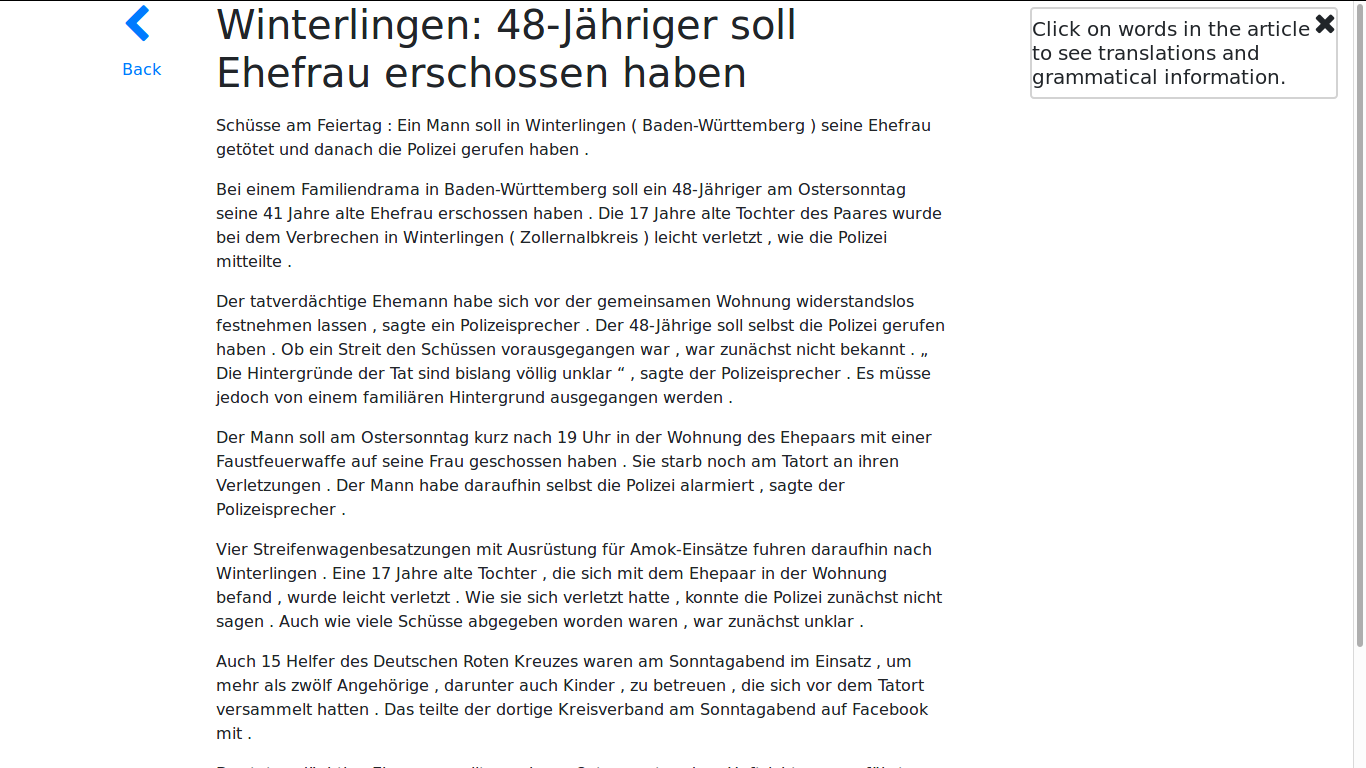
\includegraphics[width=0.7\textwidth]{Graphics/View3}
\end{center}
\end{figure}

Clicking on a word on the article, will make a gloss item appear on the right of the screen, making the screen appear similar to the view shown in Figure \ref{fig:view4}. This positioning makes it marginal gloss, which was found to be effective by \textcite{abuseileek2008}. New items appear at the bottom of the margin and will stay in the margin until they are dismissed by the user. If there are too many gloss entries for the screen, then a scroll bar will appear allowing the user to scroll through the gloss entries independent of that user's scrolling through the article content. The gloss entries are permanent until dismissed as this prevents the user from having to lookup the same word multiple times.

\begin{figure}
	\caption[Screenshot of the Article Reading View with Gloss]{Another screenshot of the article reading view, this time with a gloss entry in the margin.}
	\label{fig:view4}
	\begin{center}
	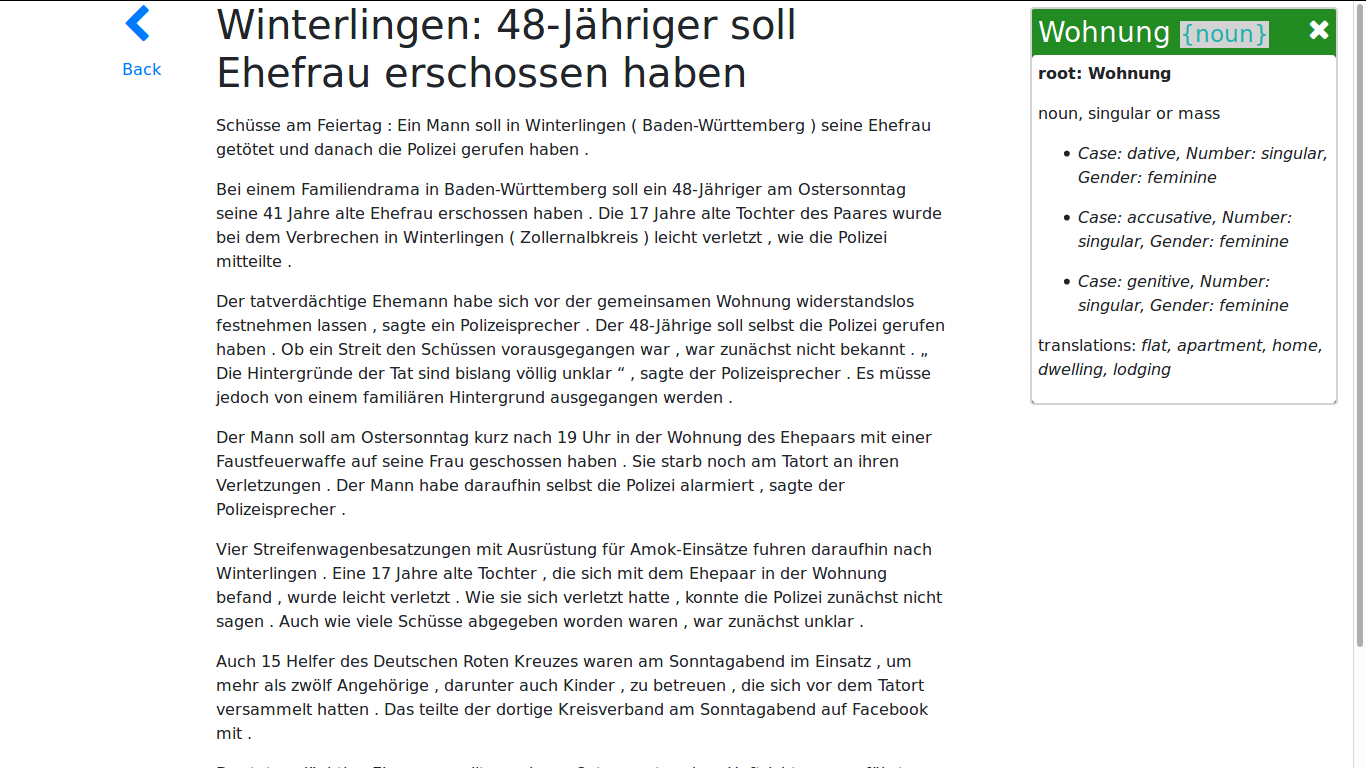
\includegraphics[width=\textwidth]{Graphics/View4}
\end{center}
\end{figure}
 
\subsection{Gloss Items}

\begin{figure}
	\caption{Screenshot of a Gloss Entry}
	\label{fig:gloss}
	\begin{center}
	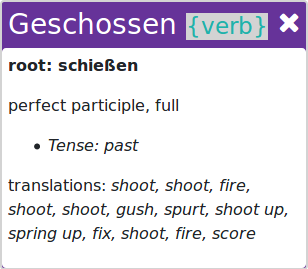
\includegraphics[width=0.3\textwidth]{Graphics/Gloss}
\end{center}
\end{figure}

The design of the gloss items was inspired by the design of dictionary entries. An example gloss entry can be seen above in Figure \ref{fig:gloss}. The top of the gloss is a colour specified by the lexical category of the word; green for nouns, purple for verbs, blue for adjectives, red for any other and black for ones that cannot be identified. The header then contains the form of the words as it appears in the text, followed by the lexical category, in curly brackets, with unique text and background colours. A white cross is on the right of the header, clicking it dismisses the gloss entry, removing it from the gloss. 

The body of the gloss is divided into three parts. The root word, the grammatical information and then possible translations of the root. The root is presented at the top, in bold. This is done so that if the user can identify the word by the root, then they only need to read that. 

After the root, the grammatical information of the word. First is a short description of the word's lexical category and form of the word. Following this is a bullet point list of the possible use cases of the word in this form. Its tense and person if it's a verb, its  gender, plurality and case if it's a noun and other relevant information for the other lexical categories. 

Finally the body is concluded with various translations of the root words. In the case that the application cannot find a translation, the phrase "no translations found" is presented instead. 
 